% kompilace xelatex prezentace.tex
% dokumentace k beameru: http://ftp.cvut.cz/tex-archive/macros/latex/contrib/beamer/doc/beameruserguide.pdf

% nastavení formátu prezentace 16:9
\documentclass[czech,aspectratio=169]{beamer}

\usepackage{polyglossia}
\setmainlanguage{czech}

% nastavení vzhledu 
% další možnosti vzhledu viz https://hartwork.org/beamer-theme-matrix/
\usetheme{Berlin}
\usecolortheme{whale}

% vzhled slajdů vnitřní téma (např. vzhled odrážek)
\useinnertheme{rectangles} %možnosti: default circles rectangles rounded inmargin
% vzhled slajdů vnější téma
\useoutertheme{default} %možnosti: default, miniframes, smoothbars, sidebar, split, shadow, tree, smoothtree, infolines

% zavedeme čvutí modou barvu
\definecolor{CVUT}{HTML}{0065BD}
% čvutí modrou použijeme jako hlavní barvu prezentace
\setbeamercolor{structure}{bg=white,fg=CVUT}

% jako font prezentace nadefinujeme oficiální ČVUT písmo Technika
% https://www.cvut.cz/logo-a-graficky-manual  -- inforek, příhlášení přes celoškolské heslo
\usepackage{fontspec}
\setsansfont{Technika-Book}

% vypneme navigační panel beamer (pro zapnutí zakomentujeme)
\beamertemplatenavigationsymbolsempty

% vygenerujeme slajdy s poznámkami
%\setbeameroption{show notes} 

% vygeneruje slajdy s poznámky vhodné pro promítání na dvou monitorech
%\usepackage{pgfpages}
%\setbeameroption{show notes on second screen}

% další balíčky
\usepackage{graphicx}
\usepackage{hyperref}
\usepackage{media9}
\usepackage{multimedia}
\usepackage{tikz}
\usetikzlibrary{calc}
\usetikzlibrary{chains,fit,shapes}

% Údaje o prezentaci
\title[Webová aplikace pro online web scraping]{Webová aplikace pro online web scraping}
\subtitle{Bakalářská práce}
\institute[FIT ČVUT v Praze]{Fakulta informačních technologií \\ České vysoké učení technické v Praze}
\author[J. Drahoš]{Jakub Drahoš \\ Vedoucí práce: Mgr. Martin Podloucký}
\date{12. 5. 2019}
\titlegraphic{
\includegraphics[width=.1\textwidth]{assets/logo-cvut}}


\begin{document}
	\begin{frame}
		\titlepage
	\end{frame}

	\begin{frame}
		\tableofcontents 
	\end{frame}
	
	% ---------------------------------------------------------------------------
	
	\section{Úvod}
	\begin{frame}{Web scraping}
		\begin{itemize}
			\item = technika získávání dat z internetových stránek
			\item Většinou automatizované
			\item Např. marketingové společnosti nebo sledování produktů
		\end{itemize}
	\end{frame}

	\begin{frame}{Cíle práce}
		\begin{enumerate}
			\item Tvorba aplikace umožňující provádět web scraping
			\item Právní rešerše
			\item Analýza stávajících řešení
		\end{enumerate}
	\end{frame}

	% ---------------------------------------------------------------------------
	
	\section{Stávající řešení}
	\begin{frame}{Nevýhody konkurence}
		\begin{itemize}
			\item Složité a neintuitivní ovládání
			\item Nepřehledné grafické rozhraní
			\item Mnoho funkcionality na úkor uživatelského zážitku
		\end{itemize}
	\end{frame}

	\begin{frame}
		\begin{center}
			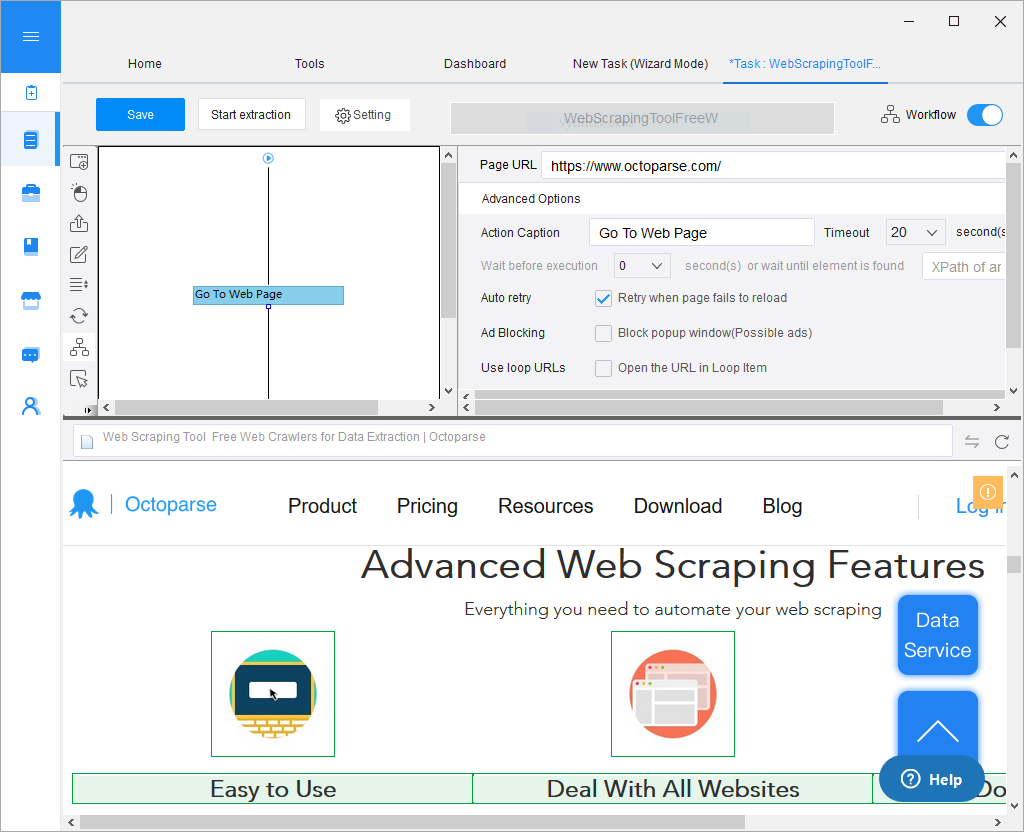
\includegraphics[width=0.6\textwidth]{assets/Octoparse.png}
		\end{center}
	\end{frame}

	\begin{frame}
		\begin{center}
			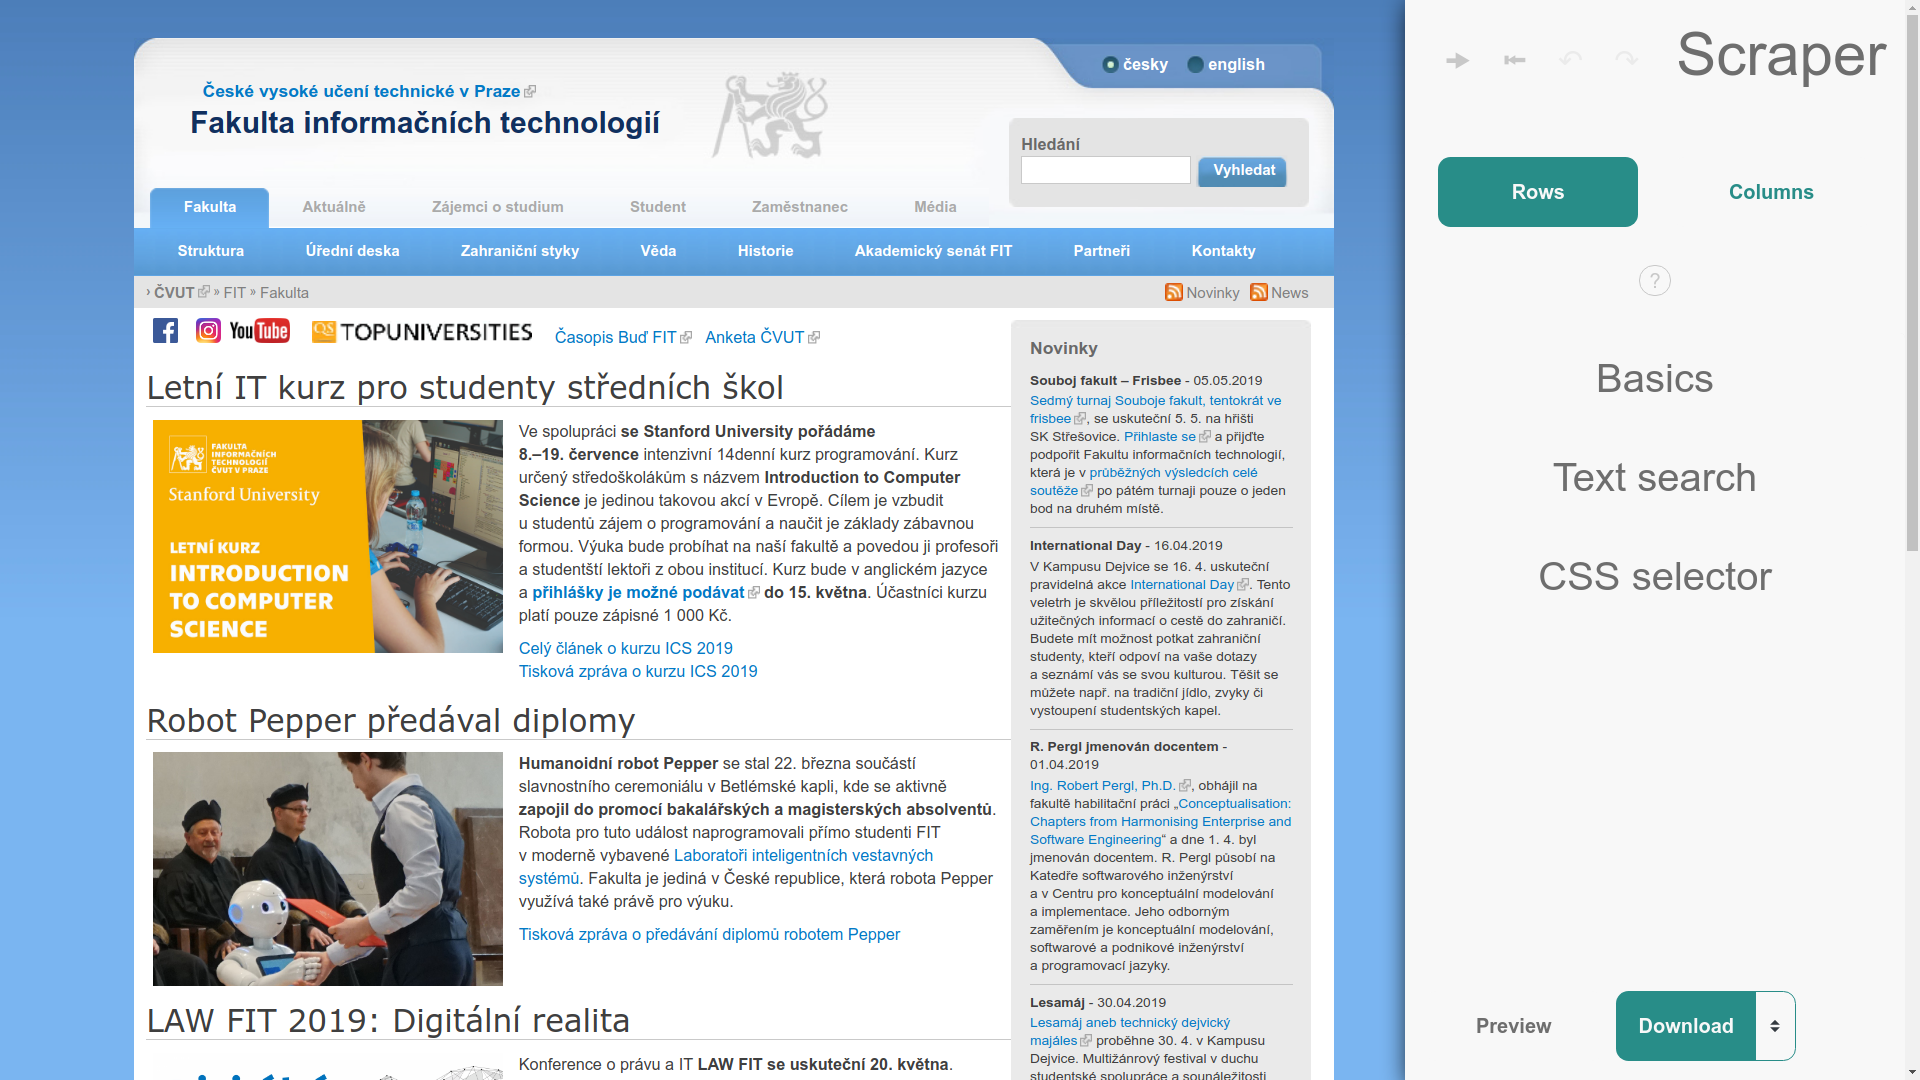
\includegraphics[width=0.85\textwidth]{assets/Scraper_control_panel.png}
		\end{center}
	\end{frame}
	
	% ---------------------------------------------------------------------------
	
	\section{Výsledná aplikace}
	\begin{frame}{Implementace}
		\begin{itemize}
			\item Implementováno jako rozšíření do prohlížeče Google Chrome
			\item Napsané v jazyce JavaScript
			\item Určené především ke statickému vytěžování stránek
		\end{itemize}
	\end{frame}

	\begin{frame}
		\begin{center}
			\includemedia[
				label=scraper,
				height=0.49\linewidth,
				activate=pageopen,
				final,
				passcontext,
				addresource=assets/ukazka2.mp4,
				flashvars={
					source=assets/ukazka2.mp4&
					autostart=true&autoPlay=true
				}
			]{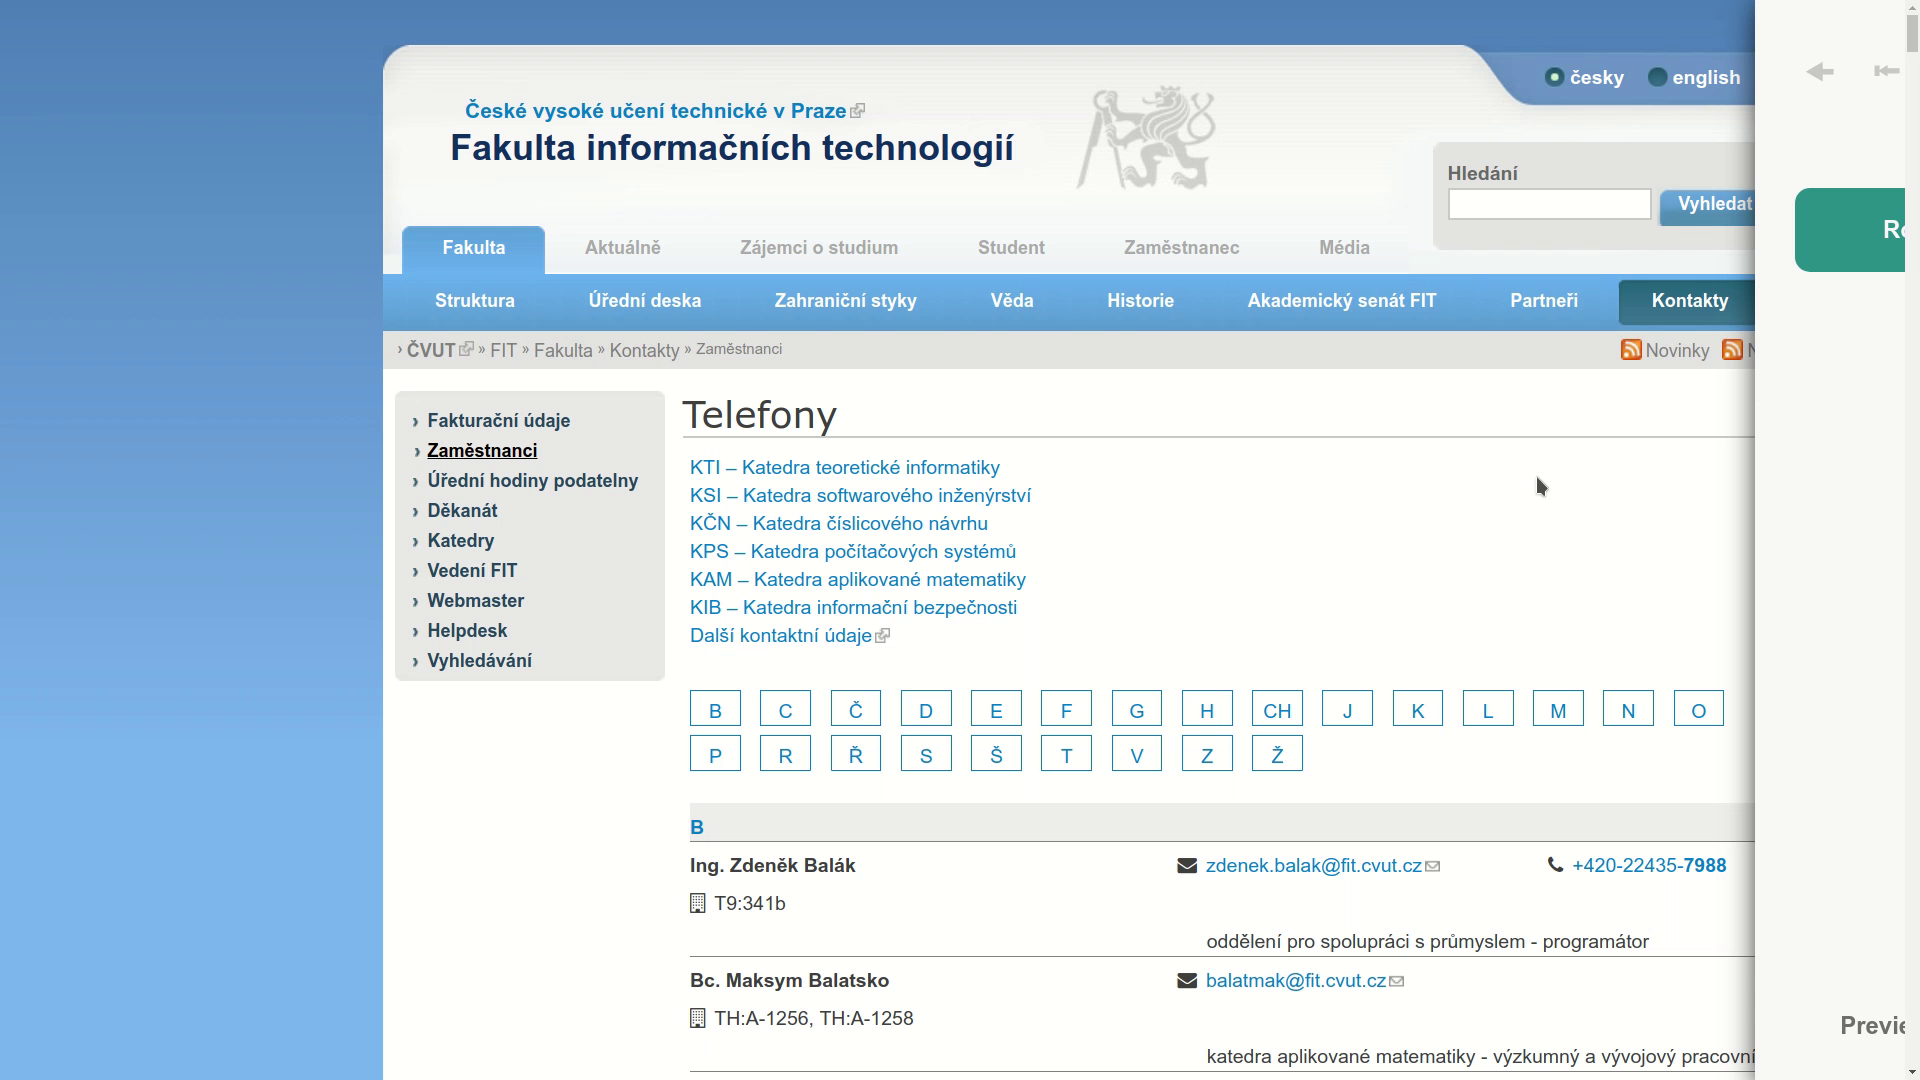
\includegraphics[height=0.49\linewidth]{assets/video_snapshot.png}}{VPlayer.swf}
		\end{center}
	\end{frame}

	\begin{frame}{Výhody oproti konkurenci}
		\begin{itemize}
			\item Jednoduchá na používání
			\item Přehledné grafické rozhraní
			\item Extrakce během pár okamžiků 
		\end{itemize}
	\end{frame}

	% ---------------------------------------------------------------------------
	
	\section{Shrnutí}
	 \begin{frame}{Shrnutí}
	 	\begin{itemize}
	 		\item Právní rozbor problematiky
	 		\item Nedostatky konkurenčních nástrojů
	 		\item Vytvoření aplikace se zaměřením na uživatelský zážitek
	 	\end{itemize}
	 \end{frame}

\end{document}
